% §4 Modelling assumptions.  A1 (GTR) and A2 (clock), the constant block model they induce at the
% root split, and the two scalars eta and rho in which the sampling rate is stated.  C1 is on its
% own counter: it is an inequality on the tree, not a hypothesis on the data.  The proof of
% prop:cfbm is deferred to app:comp1; the Fiedler-vector shape belongs to lem:A-decomp, not here.
\section{Modelling assumptions}\label{sec:assumptions}

In this section we state the two hypotheses the analysis carries, the block model they put the
similarity matrix in, and the two scalars in which the sampling rate of \Cref{sec:main} is
expressed.

\begin{assumption}[GTR substitution model]\label{asm:gtr}
The substitution model of \Cref{sec:bg-model} holds: a single GTR generator $Q$ satisfying
(i)--(iv) drives every edge.
\end{assumption}

\begin{assumption}[Molecular clock]\label{asm:clock}
Every branch of $\mathcal{T}$ has positive length, and all $m$ terminal nodes are contemporaneous:
$\tau_{x_i}=0$ for every $i$.
\end{assumption}

\Cref{asm:gtr} already removes per-lineage rate variation --- one generator, and a branch length
that is a difference of heights --- so \Cref{asm:clock} is what makes $\mathcal{T}$ ultrametric.
That is what places $S$ in the model on which spectral bipartitioning is analysed: the
\emph{constant block model} (CBM) of Balakrishnan et al.\ \cite{Balakrishnan2011clustering}, in the
localized form used for latent trees by \cite{aizenbud2023spectral}.

\begin{definition}[Constant block model at a bipartition]\label{def:cfbm}
A symmetric matrix $S$ with unit diagonal satisfies the \emph{constant block model} at a
bipartition $\mathcal{X} = C_1 \cup C_2$ if its cross-block entries share one value
$\bze\in(0,1)$ and every within-block entry exceeds it:
\begin{equation}\label{eq:cfbm_floor}
   S_{ij}=\bze\quad(i\in C_1,\ j\in C_2),
   \qquad
   \bze<\Sin^{\min}\le S_{ij}\le\Smax<1\quad(i\ne j\ \text{in one block}),
\end{equation}
where $\Sin^{\min}$ and $\Smax$ are the extreme within-block entries. The blocks themselves are
arbitrary.
\end{definition}


\begin{proposition}[The population similarity is a constant block model at the root split]\label{prop:cfbm}
Under \Cref{asm:gtr,asm:clock}, the population similarity matrix of \Cref{def:simgraph} satisfies
\Cref{def:cfbm} at the root split $\mathcal{X}=C_1\cup C_2$, whose blocks are complementary clades
of $\mathcal{T}$, with
\begin{equation}\label{eq:cfbm_from_model}
   \bze = \exp\bigl(2\,\mathrm{tr}(Q)\,\tau_r\bigr),
   \qquad
   \Sin^{\min} = \exp\bigl(2\,\mathrm{tr}(Q)\,\tau^{\max}\bigr),
\end{equation}
for $\tau_r$ the root height and $\tau^{\max}<\tau_r$ the greatest within-clade MRCA height.
\end{proposition}

\noindent \Cref{app:comp1} proves it. With the terminal nodes ordered along the split as in
\Cref{sec:bg-model}, the matrix and its Laplacian take the block form
\begin{equation}\label{eq:block_forms}
   S=\begin{pmatrix} S_{C_1} & \bze J_{|C_1|\times|C_2|}\\ \bze J_{|C_2|\times|C_1|} & S_{C_2}\end{pmatrix},
   \qquad
   L=\begin{pmatrix} D_{C_1}-S_{C_1} & -\bze J_{|C_1|\times|C_2|}\\ -\bze J_{|C_2|\times|C_1|} & D_{C_2}-S_{C_2}\end{pmatrix},
\end{equation}
with $J$ the all-ones block and the block degrees
$D_{C_1}=\operatorname{diag}(S_{C_1}\1_{|C_1|})+|C_2|\bze I_{|C_1|}$,
$D_{C_2}=\operatorname{diag}(S_{C_2}\1_{|C_2|})+|C_1|\bze I_{|C_2|}$. The diagonal blocks are
whatever the two subtrees make them; only the off-diagonal block is pinned, and that is the single
structural fact the spectral analysis of \Cref{sec:bridging} runs on.

Two scalars carry the split through the analysis: how unevenly it divides the terminal nodes, and
how sharply within-block similarities exceed cross-block ones.

\begin{definition}[Imbalance ratio and structural margin]\label{def:imbalance}
For block sizes $|C_1| \le |C_2|$ with $|C_1|+|C_2|=m$, the \emph{imbalance ratio} is
\begin{equation}\label{eq:imbalance_ratio}
   \eta:=\frac{|C_2|}{|C_1|}\ \ge\ 1 .
\end{equation}
With $\bze$ and $\Sin^{\min}$ as in \eqref{eq:cfbm_floor}, the \emph{structural margin} is the
amount by which the weakest within-block similarity clears the cross-block baseline,
\begin{equation}\label{eq:margin_definition}
   \rho := \Sin^{\min}-\bze \ >\ 0 .
\end{equation}
\end{definition}

\noindent A balanced split has $\eta=1$, while caterpillar-like lineages reach
$\eta=\mathcal{O}(m)$. The pair plays the role of the two constants of Balakrishnan et al.\
\cite{Balakrishnan2011clustering}: $\eta$ is their balanced-cluster constant and $\rho$ their
separation gap. Because \Cref{def:cfbm} pins every cross-block entry to the single value $\bze$,
the range restriction of that work contributes no further term to $\rho$ here.

\Cref{asm:gtr,asm:clock} are hypotheses on how the data are generated, and they already fix every
quantity in \eqref{eq:margin_definition}. What they do not fix is whether those quantities stand in
the relation the analysis needs. That relation is the following inequality. It is not an assumption
about the data but a property checkable on any given tree, and it is what delimits the trees the
guarantee covers; it is the only condition beyond \Cref{asm:gtr,asm:clock} that the main result
carries.

\begin{condition}[Separation margin]\label{asm:margin}
The structural margin strictly dominates the imbalance-weighted cross-block baseline,
\begin{equation}\label{eq:margin_assumption}
   \rho>\eta\,\bze,\qquad\text{equivalently}\qquad
   \Sin^{\min}>(1+\eta)\,\bze .
\end{equation}
\end{condition}

\Cref{fig:fiedler_partitions} shows the Fiedler split on three simulated trees spanning the range of
$\eta$: the smaller the clade the rule cuts off, the larger the values its terminal nodes carry.

\begin{figure}[t]
\centering
\begin{subfigure}[t]{0.30\textwidth}
  \captionsetup{singlelinecheck=false, justification=raggedright, skip=1pt}
  \subcaption{$\eta=1.5$}\label{fig:fied-eta01}
  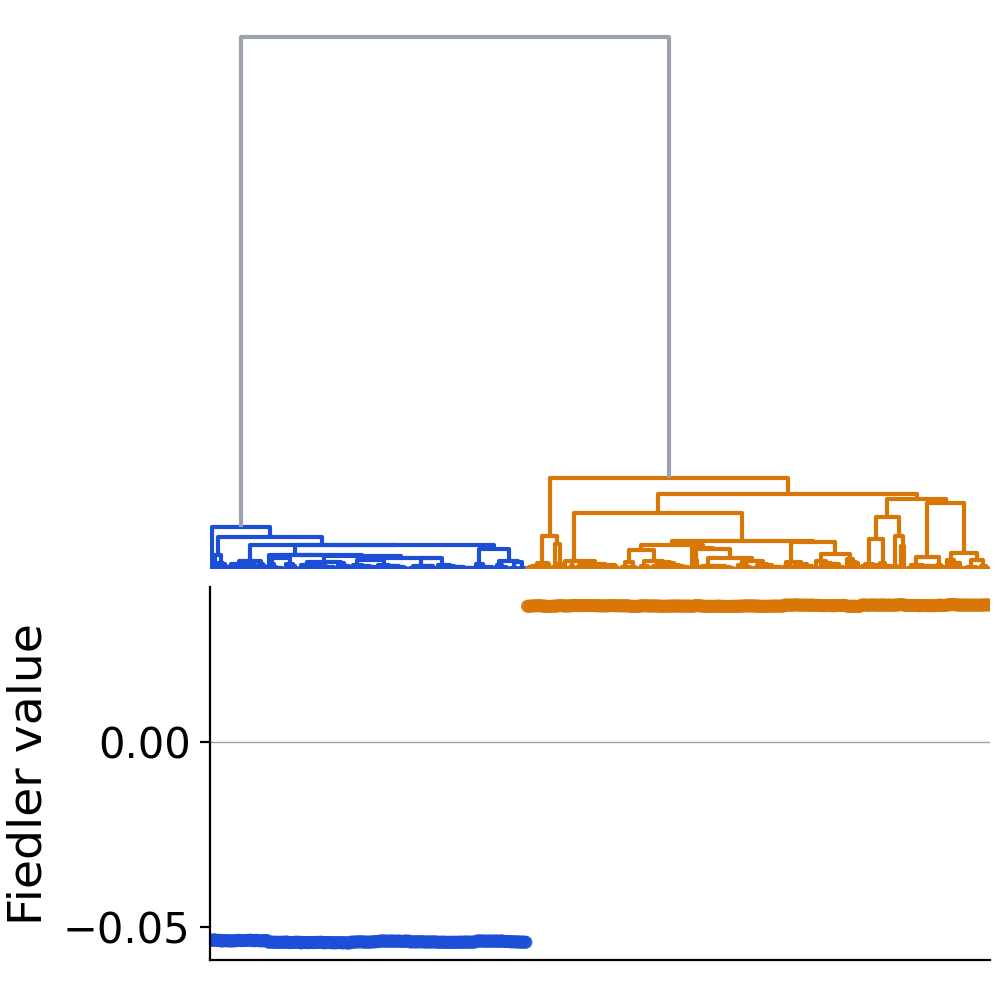
\includegraphics[width=\textwidth]{Fiedler_Bipartitions/fiedler_tree_partition_eta01.png}
\end{subfigure}
\hfill{\color{black!25}\rule[-5.0cm]{0.4pt}{5.0cm}}\hfill
\begin{subfigure}[t]{0.30\textwidth}
  \captionsetup{singlelinecheck=false, justification=raggedright, skip=1pt}
  \subcaption{$\eta=4.4$}\label{fig:fied-eta05}
  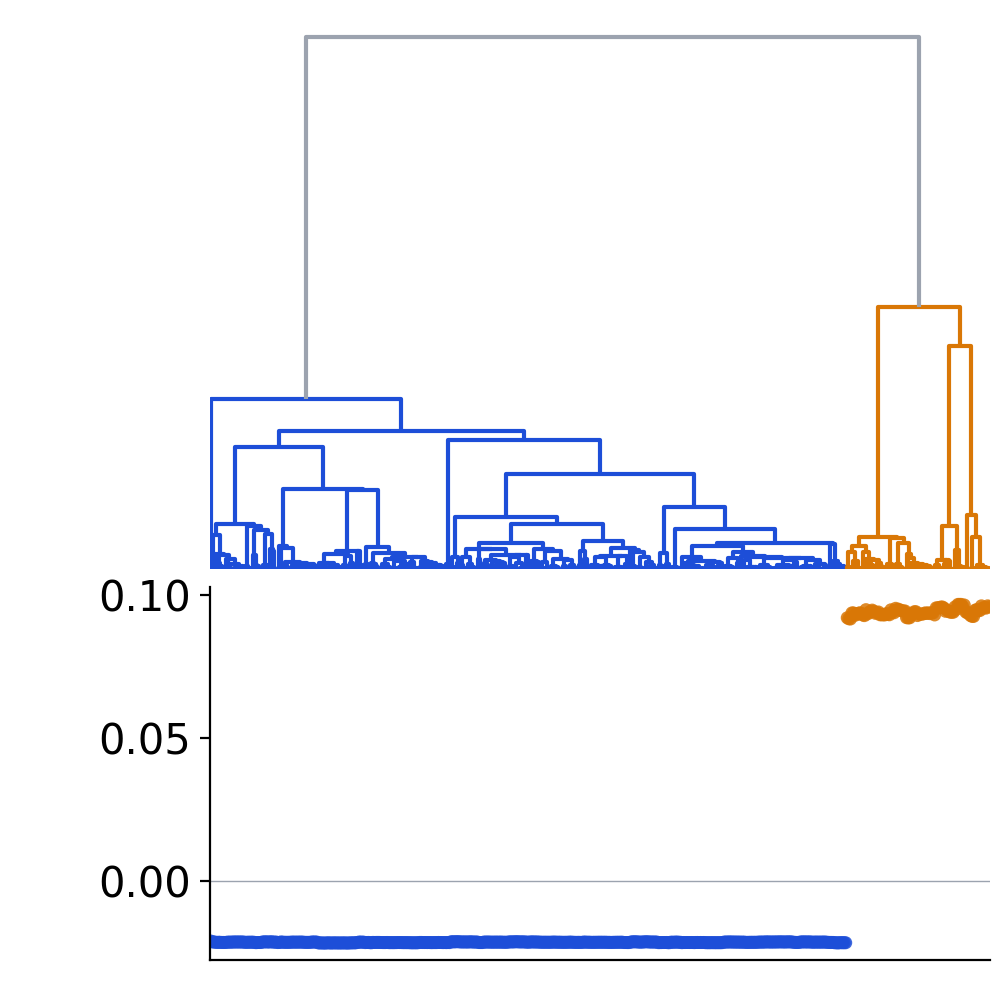
\includegraphics[width=\textwidth]{Fiedler_Bipartitions/fiedler_tree_partition_eta05.png}
\end{subfigure}
\hfill{\color{black!25}\rule[-5.0cm]{0.4pt}{5.0cm}}\hfill
\begin{subfigure}[t]{0.30\textwidth}
  \captionsetup{singlelinecheck=false, justification=raggedright, skip=1pt}
  \subcaption{$\eta=15.1$}\label{fig:fied-eta15}
  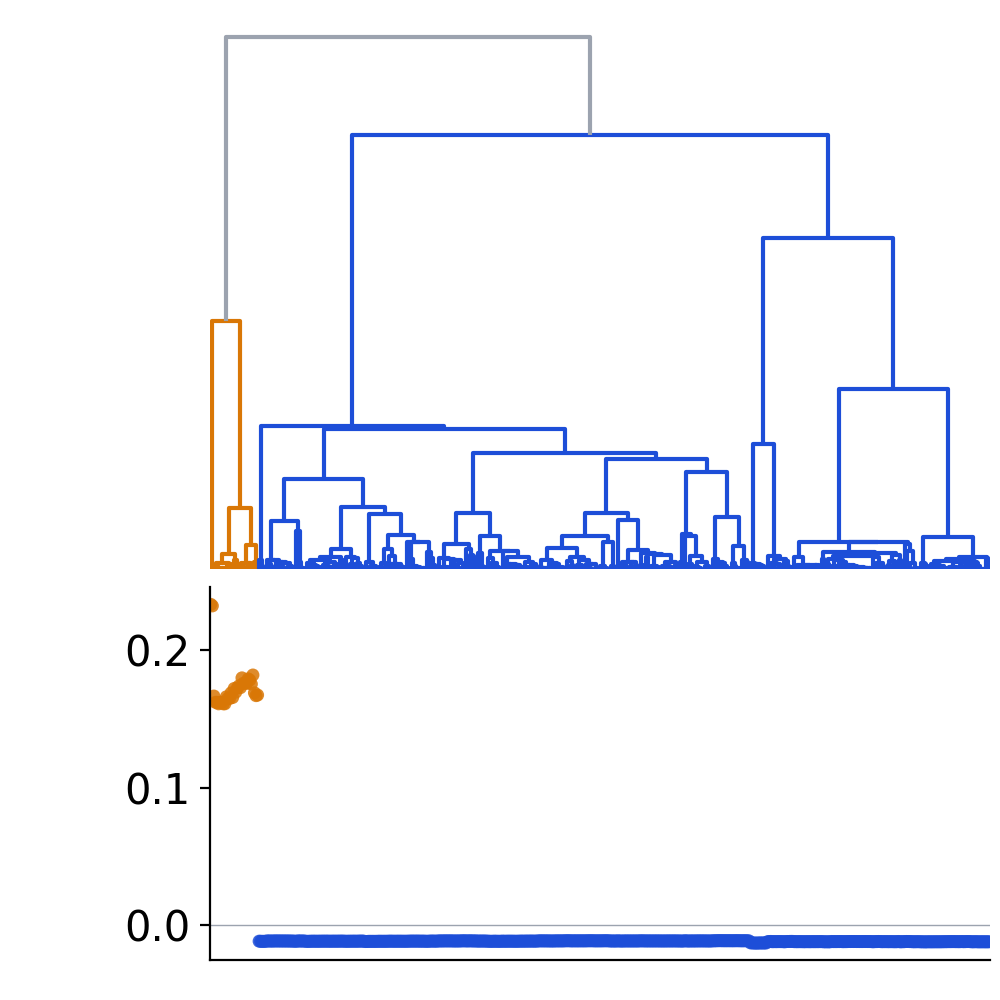
\includegraphics[width=\textwidth]{Fiedler_Bipartitions/fiedler_tree_partition_eta15.png}
\end{subfigure}
\caption{$\Pisp{S}$ on three trees, one per panel. Each is drawn
from a pool of simulated Kingman trees ($m=500$ terminal nodes, JC69 sequences of length
$\ell=10^4$) binned by the imbalance its Fiedler split realises. In each panel the
tree is on top, its branches coloured by the sign of the Fiedler vector --- grey on
the one branch that spans both signs --- and below it the Fiedler value of each terminal node
is plotted at that node's own horizontal position in the tree. The sign pattern cuts a single edge
every time, as \Cref{thm:stdr-split} requires, and the smaller the clade it cuts off, the
larger the values carried by its terminal nodes.}
\label{fig:fiedler_partitions}
\end{figure}
